%%%%%%%%%%%%%%%%%%%%%%%%%%%%%%%%%%%%%%%%%%%%%%%%%%%%%%%%%%%%%%%%%%%%%%
%% all the formatting stuff and packages

\documentclass[11pt]{article}

\parindent0em
\parskip.5em

\usepackage{xstring}

\usepackage{amsthm}
\usepackage[utf8]{inputenc}
\usepackage[ttscale=.85]{libertine}
\usepackage{libertinust1math}
% \usepackage[libertine,cmintegrals,cmbraces,vvarbb]{newtxmath}
\usepackage[T1]{fontenc}
\usepackage{microtype}
\usepackage{amsmath}
\usepackage{amssymb}
\usepackage{xspace}
\usepackage{ngerman}
\usepackage{graphicx}
\usepackage{lastpage}
\usepackage{ifthen}
\usepackage{fp}
\usepackage{hyperref}
\usepackage{icomma}
\usepackage{paralist}
\usepackage[ngerman,onelanguage,noend]{algorithm2e}
\DontPrintSemicolon

\makeatletter
\DeclareRobustCommand{\bfseries}{%
   \not@math@alphabet\bfseries\mathbf
   \fontseries\bfdefault\selectfont
   \boldmath
}
\makeatother

\usepackage[headsep=1cm]{geometry}

\usepackage{fancyhdr}

\fancypagestyle{plain}{%
  \renewcommand{\headrulewidth}{0pt}%
  \fancyhf{}
  \rhead{
\includegraphics[width = 2.4cm]{fig/hpi_logo.pdf}}
  \lhead{\textbf{\sffamily Parametrisierte Algorithmen} \\
    \textbf{\sffamily Wintersemester 2017/2018} \\
    \sffamily Thomas Bläsius}
  \cfoot{\thepage}
  \rfoot{\ifthenelse{\thepage < \pageref{LastPage}}{\textit{bitte
        wenden}}{}}
}
\fancypagestyle{normal}{%
  \renewcommand{\headrulewidth}{0pt}%
  \fancyhf{}
  \cfoot{\thepage}
  \rfoot{\ifthenelse{\isodd{\thepage} \and \thepage <
      \pageref{LastPage}}{\textit{bitte wenden}}{}}
}

\usepackage{titlesec}

\titleformat{\section}%
[hang]%
{\Large\bfseries\sffamily}%
{Aufgabe \thesection:}%
{.5em}%
{}%
[]

\renewcommand{\thesubsection}{\alph{subsection}}
\usepackage{titlesec}
\titleformat{\subsection}%
[runin]%
{\bfseries\sffamily}%
{Teilaufgabe (\thesubsection)}%
{0pt}%
{}%
[]

\usepackage{titlesec}
\titleformat{\subsubsection}%
[hang]%
{\large\bfseries\sffamily}%
{\thesection}%
{.5em}%
{}%
[]

\titlespacing{\section}{0pt}{1.5ex}{.5ex}

\titlespacing{\subsection}{0pt}{.5ex}{.5em}

\titlespacing{\subsubsection}{0pt}{1ex}{.5ex}


%%%%%%%%%%%%%%%%%%%%%%%%%%%%%%%%%%%%%%%%%%%%%%%%%%%%%%%%%%%%%%%%%%%%%%
%% commands to use in the exercise sheet/solution

\newcommand{\sheet}[2]{ %
  \title{\textbf{\sffamily Übungsblatt #1}\\[-0.5ex]
    {\normalsize \sffamily Abgabe bis #2}}
  \date{}
  \maketitle
  \pagestyle{normal}
  \vspace{-2cm}
}

\newcommand{\solution}[2]{ %
  \title{\textbf{\sffamily Musterlösung zum Übungsblatt #1}\\[-0.5ex]
    {\normalsize \sffamily Erstellt von #2}}
  \date{}
  \maketitle
  \pagestyle{normal}
  \vspace{-2cm}
}

\newcommand{\exercise}[2][]{%
  \section{#2 \hfill {\normalsize#1}}%
}

\newcommand{\subexercise}{%
  \subsection{}%
}

\newcommand{\how}[1]{%
  \subsubsection*{Wie kommt man drauf?}%
}




\DeclareMathOperator{\vc}{vc}

\begin{document}

\solution{1}{Thomas Bläsius und Philipp Fischbeck}

\exercise{Verschiedenes}

\subexercise

Ja, denn $2^{\Theta(n)}$ kann beispielsweise für $2^{2n} = 4^n$
stehen, was asymptotisch echt schneller wächst als $2^n$.  Umgekehrt
beinhaltet $2^{\Theta(n)}$ auch
$2^{n/2} = (\sqrt{2})^n \approx 1,41^n$, was langsamer wächst als
$2^n$.  Man kann also nicht sagen, dass $2^{\Theta(n)}$ langsamer oder
schneller wächst als $\Theta(2^n)$.  Allerdings ist $2^{\Theta(n)}$
ungenauer.

\subexercise

Da $T$ ein Baum ist, gilt $m = n-1 = n_1 + n_3 - 1$.  Außerdem ist die
Summe der Knotengrade $2m$, also $2m = n_1 + 3n_3$.  Ersetzt man $m$
in der zweiten Gleichung durch die erste, so erhält man
%
\begin{align*}
  2(n_1 + n_3 - 1) & = n_1 + 3n_3,\\
  2n_1 + 2n_3 - 2 & = n_1 + 3n_3, \\
  n_1 - 2         & = n_3.
\end{align*}

\subexercise

Angenommen, ein Problem $P$ mit Parameter $k$ ist für konstantes $k$
NP-vollständig.  Dann würde ein FPT-Algorithmus für dieses
parametrisierte Problem $\mathrm{P} = \mathrm{NP}$ implizieren.
Umgekehrt würde $\mathrm{P} = \mathrm{NP}$ implizieren, dass $P$ in
polynomieller Zeit (und damit insbesondere in FPT-Zeit) lösbar ist.
Man muss also nur parametrisierte Probleme finden, die für einen
konstanten Parameter schon NP-vollständig sind.  Hier ein paar Beispiele:
%
\begin{itemize}
\item $k$-\textsc{Sat} (jede Klausel enthält $k$ Literale) mit dem
  Parameter $k$ ist für $k = 3$ NP-vollständig.
\item $k$-\textsc{Färbung} in Graphen mit dem Parameter $k$ ist für
  $k = 3$ schon NP-vollständig.
\item \textsc{Hamilton Pfad} in Graphen mit dem Maximalgrad $k$ als
  Parameter ist für $k = 3$ schon NP-vollständig.
\end{itemize}



\exercise{Untere Schranken für \textsc{RegEx}}
Betrachte den regulären Ausdruck
$R_n = (0\cup 1)^\star 1 (0\cup 1) \dots (0\cup 1)$, wobei der
Teilausdruck $(0\cup 1)$ $\frac{n}{6}$-mal wiederholt wird.  Damit gilt
$|R_n| = \frac{5}{6}n + 7$, was für ausreichend großes $n$ echt
kleiner als $n$ ist.  Für $T_n$ wähle einen beliebigen String, sodass
$|R_n| + |T_n| = n$.  Damit erhalten wir die unendliche Familie von
\textsc{RegEx}-Instanzen
$\{(R_n, T_n) \mid n \text{ ausreichend groß}\}$.

Wir zeigen, dass jeder zu $R_n$ äquivalente DEA mindestens $2^{n/6}$
Zustände hat.  Damit benötigt die Berechnung des DEA's $2^{\Omega(n)}$
Zeit (unabhängig von $|T|$).  Der DEA muss genau die Wörter über
$\Sigma = \{0, 1\}$ akzeptieren, die an der $n/6+1$-ten Stelle von
hinten eine $1$ haben.  Betrachte zwei Wörter $w_1\not= w_2$ der Länge
$n/6$.  Angenommen, $w_1$ und $w_2$ unterscheiden sich an der $k$-ten
Stelle und sei ohne Beschränkung der Allgemeinheit $w_1[k] = 1$ und
$w_2[k] = 0$.  Liest der DEA nach Abarbeitung von $w_1$ noch das Wort
$0^{k}$ bestehend aus $k$ $0$-en, so muss der DEA akzeptieren, da die
$n/6+1$-te Stelle von hinten gerade $w_1[k] = 1$ ist.  Für $w_2$ darf
der DEA bei gleichem Vorgehen nicht akzeptieren.  Nach Abarbeitung
zweier unterschiedlicher Wörter $w_1 \not= w_2$ der Länge $n/6$ muss
sich der DEA also in unterschiedlichen Zuständen befinden.  Da es
$2^{n/6}$ solche Wörter gibt, muss es mindestens so viele Zustände
geben.

\how

Da die Simulation eines Wortes auf dem DEA schnell geht, muss die
exponentielle Laufzeit in der Konstruktion des DEAs stecken.  Ziel ist
es also, einen NEA zu konstruieren, sodass der dazugehörige DEA
exponentiell viel mehr Zustände benötigt.  Dieses potentiell
exponentielle Wachstum von NEA zu DEA kommt daher, dass sich ein NEA
zu jedem Zeitpunkt in einer Teilmenge der Zustände befinden kann.  Man
muss also dafür sorgen, dass exponentiell viele solcher Teilmengen
auch möglich sind.  Um das zu erreichen, kann man folgende zweiteilige
Idee benutzen.  Man sorgt dafür, dass es einen Zustand $q_1$ gibt, der
genau dann erreichbar ist, wenn gerade eine $1$ gelesen wurde.  Damit
kann man die Erreichbarkeit von $q_1$ leicht durch die Eingabe
kontrollieren.  Baut man nun noch eine Kette, die den Status von $q_1$
(also ob $q_1$ erreichbar ist oder nicht) in jedem Schritt eins weiter
gibt, so kann man diesen Status für jeden Zustand in der Kette
individuell belegen, indem man die entsprechende Eingabe wählt.  Man
kann also für jede Teilmenge dieser Zustände eine Eingabe finden, die
genau diese Teilmenge erreichbar macht. Setzt man das zusammen,
erhält man den unten abgebildeten NEA, der dem regulären Ausdruck in
der Lösung oben entspricht.

\begin{center}
  \vspace{1ex}
  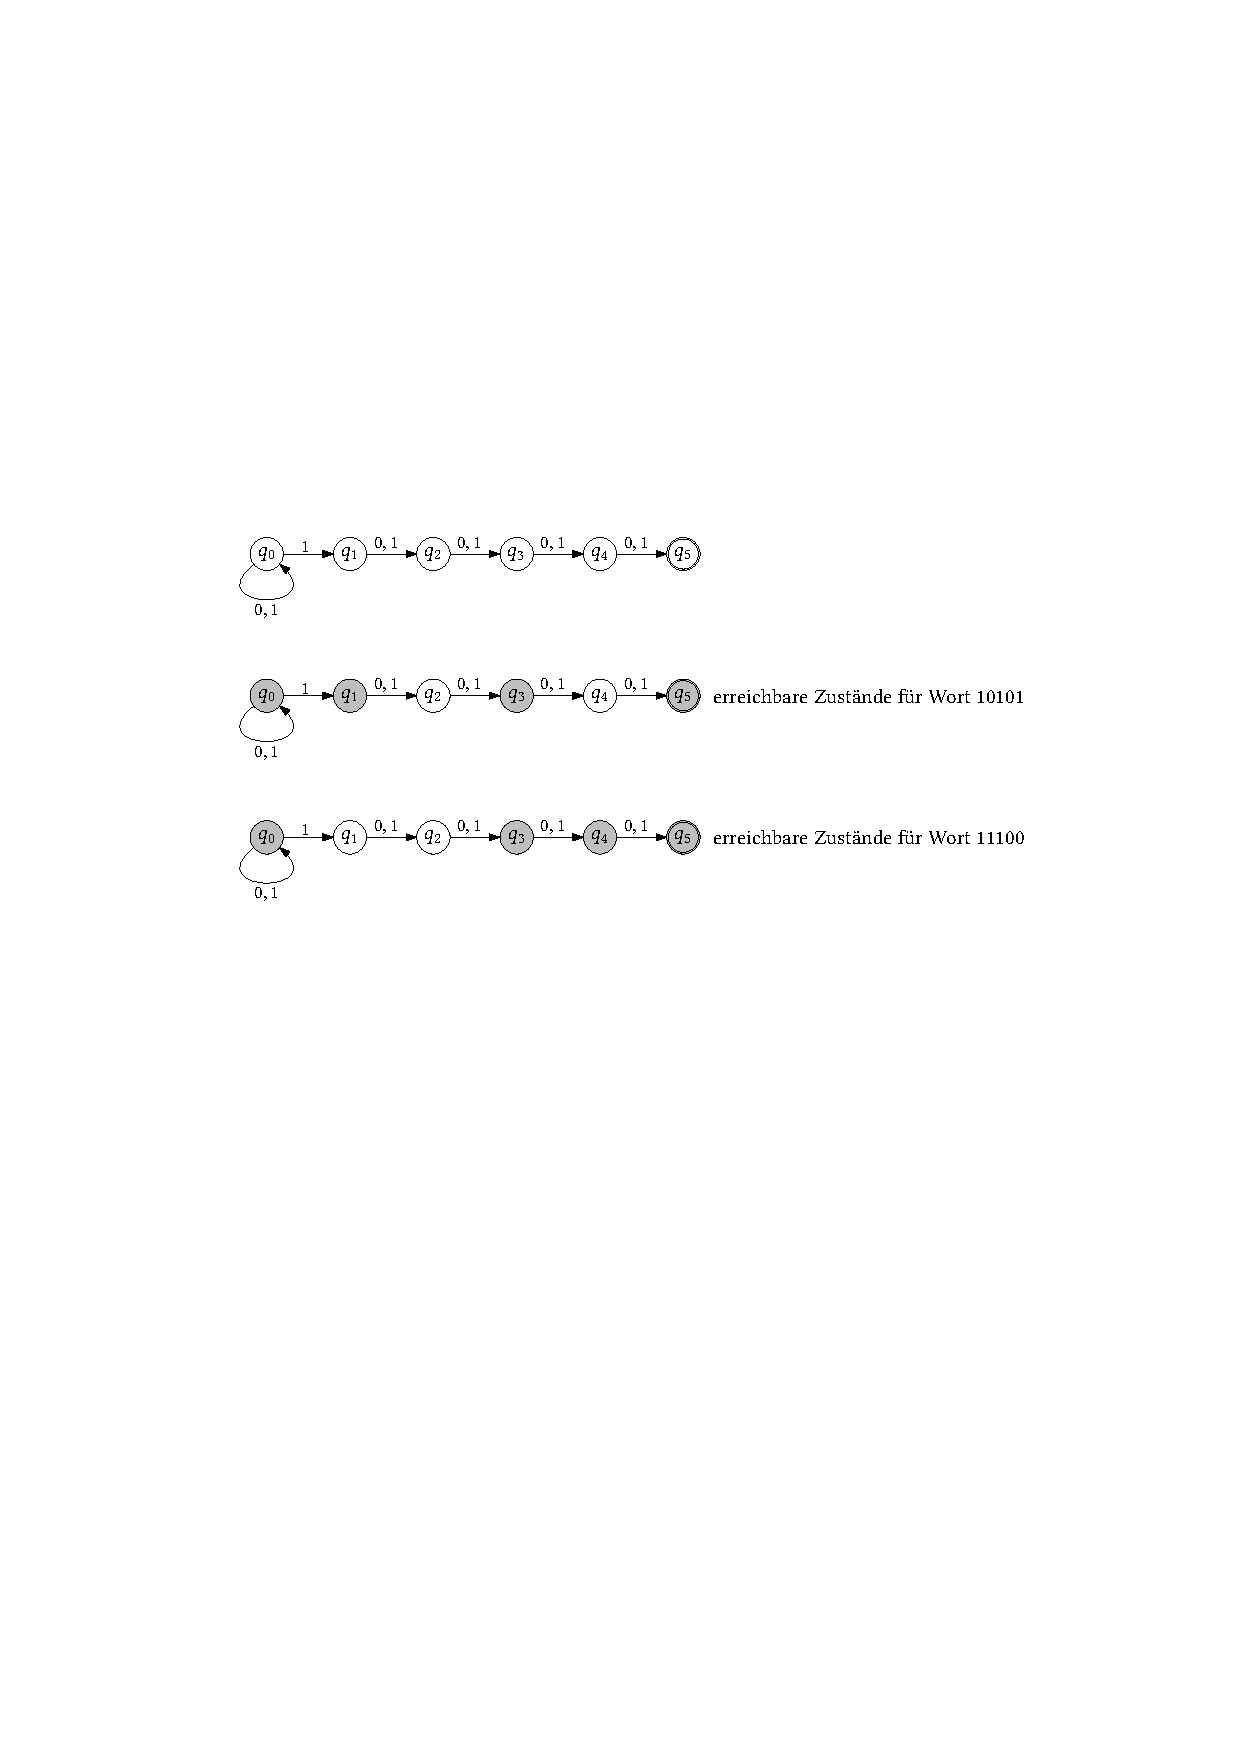
\includegraphics[page=1]{fig/01-NEA}
\end{center}

\exercise{\textsc{Vertex Cover} in speziellen Graphen}

\subexercise
\label{sec:vc-tree}

Sei $v$ ein Blatt in dem Baum (also ein Knoten mit Grad~$1$) und sei
$u$ sein Nachbar.  Da die Kante $\{u, v\}$ abgedeckt werden muss, muss
mindestens einer der beiden Knoten in der Lösung enthalten sein.  Da
$v$ keine Kanten abdeckt, die nicht auch von $u$ abgedeckt wird,
machen wir keinen Fehler, indem wir $u$ zum Vertex Cover hinzufügen.
Danach können wir $u$ und $v$ aus dem Baum löschen und mit dem Rest
genauso fortfahren.  Der Algorithmus hat offensichtlich polynomielle
Laufzeit, lässt sich aber nicht auf die gewichtete Variante
verallgemeinern.

Für die gewichtete Variante mit Gewichtsfunktion $w$ nimm an, dass der Baum gewurzelt ist
(sonst wähle eine beliebige Wurzel).  Für einen Knoten $v$ sei $T_v$
der Teilbaum bestehend aus $v$ und allen Nachfolgern von~$v$.
Bezeichne mit $\vc_-(T_v)$ das Gesamtgewicht des minimalen Vertex Covers in
$T_v$, das den Knoten $v$ nicht enthält, und mit $\vc_+(T_v)$ das Gesamtgewicht des minimalen Vertex Covers in
$T_v$, das den Knoten $v$ enthält.  Diese beiden Werte können nun wie
folgt mit einem dynamischen Programm berechnet werden.  Seien
$v_1, \dots, v_k$ die Kinder von $v$. 
Wenn $v$ in dem Vertex Cover für $T_v$ enthalten ist, so kann man für
die Teilbäume $T_{v_i}$ beliebige Vertex Cover wählen und wählt daher jeweils das mit kleinerem Gesamtgewicht.  Es gilt also
$\vc_+(T_v) = w(v) + \min\{\vc_-(T_{v_1}), \vc_+(T_{v_1})\} + \dots + \min\{\vc_-(T_{v_k}), \vc_+(T_{v_k})\}$.  Wenn $v$
nicht in dem Vertex Cover enthalten ist, dann müssen sämtliche
Kinder von $v$ enthalten sein.  Es gilt also
$\vc_-(T_v) = \vc_+(T_{v_1}) + \dots + \vc_+(T_{v_k})$.

Wenn $r$ die Wurzel ist, so liefert $\min\{\vc_+(T_r), \vc_-(T_r)\}$ nach
Beendigung des dynamischen Programms das Vertex Cover mit minimalem Gesamtgewicht.
Diese Lösung funktioniert mit Knotengewichten genau wie ungewichtet (dann ist $w(v) = 1$).

\subexercise
\label{sec:vc-path}

Für $i \ge k$, sei $V_i = \{v_1, \dots, v_i\}$ die Menge der ersten
$i$ Knoten und sei $G_i$ der von $V_i$ induzierte Teilgraph.  Sei
$V_i^k = \{v_{i-k+1}, \dots, v_i\}$ die Menge der $k$ letzten Knoten
in $V_i$.  Für eine Teilmenge $S \subseteq V_i^k$, bezeichnen wir mit
$\vc_S(G_i)$ die Größe des minimalen Vertex Covers von $G_i$, das alle Knoten
aus $S$ und keinen Knoten aus $V_i^k\setminus S$ enthält.  Wenn es ein
solches Vertex Cover nicht gibt (weil es zwei verbundene Knoten in
$V_i^k\setminus S$ gibt), dann setzen wir formal
$\vc_S(G_i) = \infty$.  Ähnlich wie in Aufgabenteil~\ref{sec:vc-tree}
benutzen wir ein Dynamisches Programm, um diese Information für jeden
Graphen $G_i$ (startend bei $G_k$) und jede Teilmenge $S$ von $V_i^k$
zu berechnen.

Zunächst berechnen wir die $\vc$-Werte für $G_k$.  Da $G_k$ nur $k$
Knoten enthält, geht das in $O(2^k)$.  Angenommen, wir haben die
vc-Werte für $G_{i-1}$ berechnet und wollen sie jetzt für $G_i$
berechnen.  Neu hinzu kommt also der Knoten $v_i$.  Um aus einem
Vertex Cover für $G_{i-1}$ eines für $G_i$ zu machen, müssen wir
darfür sorgen, dass jede der neuen Kanten (inzident zu $v_i$)
abgedeckt ist.  Beachte, dass alle Nachbarn von $v_i$ in $V_i^k$
liegen, da keine Kante länger als $k$ ist.  Betrachte nun eine
Teilmenge $S \subseteq V_i^k$.  Ziel ist es, $\vc_S(G_i)$ zu
berechnen.  Sei $j = i-k$, d.h.\ $v_j$ ist der Knoten, der gerade so
nicht mehr zu $V_i^k$ (aber noch zu $V_{i-1}^k$) gehört.  Es gibt
dabei zwei Möglichkeiten.

\begin{enumerate}[1.]
\item Angenommen $v_i \in S$.  Dann werden alle neuen Kanten abgedeckt
  und wir erhalten
  $\vc_S(G_i) = \min\{\vc_{S - v_i}(G_{i-1}), \vc_{S - v_i +
    v_j}(G_{i-1})\} + 1$.
\item Angenommen $v_i \notin S$.  Wenn $v_i$ in $V_i^k$ einen Nachbarn
  hat, der nicht in $S$ liegt, dann gibt es kein Vertex Cover, das $S$,
  aber keinen Knoten aus $V_i^k\setminus S$ enthält.  Also erhalten
  wir $\vc_S(G_i) = \infty$.  Andernfalls erhalten wir
  $\vc_S(G_i) = \min\{\vc_{S}(G_{i-1}), \vc_{S + v_j}(G_{i-1})\}$.
\end{enumerate}

Haben wir diese $\vc$-Werte für $G_n$ berechnet, so liefert der
minimale davon das minimale Vertex Cover.  Die Laufzeit kann man grob
wie folgt abschätzen.  Im Schritt von $G_{i-1}$ zu $G_i$ benötigen wir
$O(n)$ pro Teilmenge $S \subseteq V_i^k$.  Da es $2^k$ solcher
Teilmengen gibt, benötigt der Schritt $O(2^kn)$ Zeit.  Da wir insgesamt
$O(n)$ Schritte haben, erhalten wir einen FPT-Algorithmus mit Laufzeit
$O(2^kn^2)$.


\how

In Aufgabenteil~\ref{sec:vc-tree} muss man sich fragen, was Bäume für
spezielle Eigenschaften haben, die einem helfen.  Hier können zwei
Eigenschaften helfen (daher die zwei alternativen Lösungen).  Zum
einen hat jeder Baum immer ein Blatt, wodurch man sich von den
Blättern aus durch den Baum fressen kann und zu jedem Zeitpunkt nur
ein Blatt anschauen muss.  Auf der anderen Seite funktionieren
dynamische Programme meist sehr gut auf Bäumen.  Das liegt daran, dass
man Teillösungen von Teilbäumen oft leicht kombinieren kann, weil die
Teilbäume sich nur einen Knoten teilen.

Dann muss man sich noch überlegen, welche Informationen man für die
Teilbäume kennen möchte, um daraus dieselbe Information wieder für den
größeren Teilbaum zu berechnen.  Dabei ist es recht vielversprechend,
erstmal mit so wenig Informationen wie möglich anzufangen, um dann bei
Bedarf weitere hinzuzufügen.  Konkret möchten wir für den gesamten
Baum ein minimales Vertex Cover.  Es bietet sich also an, für jeden
Knoten $v$ ein minimales Vertex Cover für den Teilbaum $T_v$ zu
berechnen.  Angenommen wir haben diese minimalen Vertex Covers für
$T_{v_1}, \dots, T_{v_k}$ berechnet, wobei $v_1, \dots, v_k$ die
Kinder von $v$ sind.  Bekommen wir daraus ein minimales Vertex Cover
für $T_v$?  Wenn wir die minimalen Vertex Cover für die Teilbäume
$T_{v_1}, \dots, T_{v_k}$ kombinieren und $v$ noch hinzu nehmen,
erhalten wir auch wieder ein minimales Vertex Cover.  Es hätte aber
ggf.\ besser sein können, $v$ nicht zu wählen.  Um diesen Fall auch
abzudecken, müssen wir uns wünschen, dass wir für jedes $T_{v_i}$
zusätzlich das minimale Vertex Cover kennen, das den Knoten $v_i$
enthält.  Damit können wir dann das minimale Vertex Cover für $T_v$
berechnen.  Aber da wir uns ja noch zusätzlich Informationen gewünscht
haben, müssen wir eben diese auch berechnen (also ein minimales
Vertex Cover von $T_v$, das $v$ enthält).  Glücklicherweise können wir
diese Zusatzinfo mit den Informationen, die wir uns schon gewünscht
haben, berechnen und müssen keine weiteren Informationen hinzunehmen.

Aufgabenteil~\ref{sec:vc-path} ist etwas komplizierter, funktioniert
aber nach dem gleichen Prinzip.  Angenommen, wir wollen ein
dynamisches Programm bauen, das in jedem Schritt einen Knoten
hinzufügt.  Wir starten wieder mit der minimal nötigen Information:
Für jeden der Teilgraphen $G_i$ wollen wir die Größe eines minimalen
Vertex Covers berechnen.  Wenn wir jetzt einen Knoten $v_i$ zu
$G_{i-1}$ hinzufügen, dann kann man diesen natürlich einfach auswählen
und erhält ein neues Vertex Cover, das um~$1$ größer ist.  Auch hier
könnte es aber wieder besser sein, den neuen Knoten $v_i$ nicht zu
wählen.  Das darf man aber nur machen, wenn das alte Vertex Cover in
$G_{i-1}$ alle Nachbarn von $v_i$ enthält.  Wir wünschen uns also als
zusätzliche Information, welche der Knoten in $G_{i-1}$ in dem Vertex
Cover enthalten sind.  Tatsächlich brauchen wir das aber nicht für
alle Knoten zu wissen, sondern nur für solche, die noch Nachbarn
außerhalb von $G_{i-1}$ haben.  Da wir $G_{i-1}$ noch nicht ansehen
können, welche Kombination dieser Knoten besonders gut für den
restlichen Graphen ist, speichern wir uns für jede Kombination ein
minimales Vertex Cover.  Da wir wissen, dass maximal die letzten $k$
Knoten in $G_{i-1}$ noch Nachbarn außerhalb von $G_{i-1}$ haben (sonst
hätten wir zu lange Kanten), müssen wir zu jedem Zeitpunkt nur $2^k$
Vertex Cover kennen.  Wie beim Baum reicht diese Information für
$G_{i-1}$ auch wieder aus, um dieselbe Information für $G_i$ zu
berechnen.

Beachte, dass das sehr ähnlich ist zu Aufgabenteil~\ref{sec:vc-tree}:
Man schaut sich die Menge der Knoten an, die noch relevant sind für
die Zukunft und berechnet für jede Teilmenge ein Vertex Cover, das die
Knoten in der Teilmenge enthält.  Beim Baum hatte diese Knotenmenge
eben die Größe~1, da für einen Teilbaum nur die Wurzel noch Kanten
nach außen hat.

\end{document}
